The above equations can be expressed in vector form as,
\begin{align}
\myvec{5 & 2}\vec{x} = 4\\
\myvec{7 & 3}\vec{x} = 5
\end{align}
Now, writing it in the matrix form as, 
\begin{align}
\myvec{5 & 2 \\ 7 & 3}\vec{x} = \myvec{4 \\ 5}
\end{align}
The augmented matrix of above equation is solved by row reduction as follows
\begin{align}
\myvec{5 & 2 & 4 \\ 7 & 3 & 5}  \xleftrightarrow[]{R_2\leftarrow R_2-\brak{\frac{7}{5}}R_1} \myvec{5 & 2 & 4 \\ 0 & \frac{1}{5} & \frac{-3}{5}}
\end{align}
\begin{align}
\xleftrightarrow[]{R_1\leftarrow R_1-10R_2} \myvec{5 & 0 & 10 \\ 0 & \frac{1}{5} & \frac{-3}{5}}
\end{align}
\begin{align}
\implies \vec{x} = \myvec{2 \\ -3}
\end{align}
See Fig. \ref{Fig 1:solutions/det/58/}

\begin{figure}
\centering
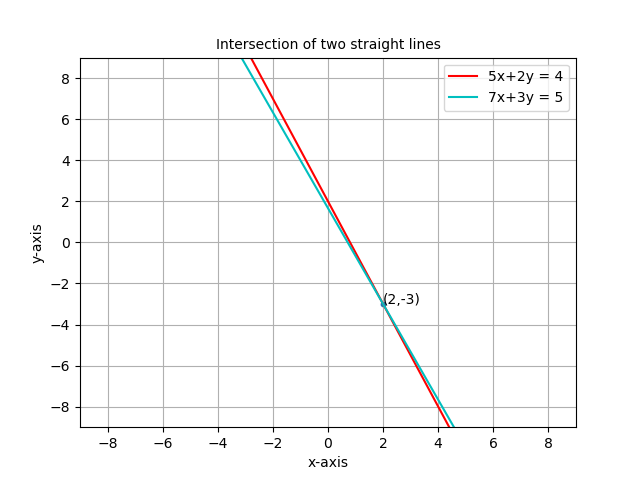
\includegraphics[width=\columnwidth]{./solutions/det/58/Figure_2.png}
\caption{Intersection of 2 lines}
\label{Fig 1:solutions/det/58/}
\end{figure}
